\section{Theory and experimental setup}

\subsection{General explanation about plasma}
Though every gas always has a small degree of ionisation, plasma has some defining qualities [which sets it apart][which require a separate description][which justify the need to properly define it [the need for a proper definition]].
[A common definition of plasma is that of a] [a simple textbook definition would be a] \emph{quasineutral} gas of charged and neutral particles which exhibits \emph{collective} behaviour \cite{chen_introduction_1990}.

The concepts of quasineutrality and collectivity need further explanation.
[While this may seem precise, we must define what quasineutral and collective means]

Quasineutrality is a mathematical way of saying that eventhough the particles making up a plasma consist of free electrons and ions, 
their overall charge densities cancel each other in equilibrium\cite{gibbon_introduction_2016}.
(La citation a aussi une formule pour expliquer).


Explain concept of Debye sphere and length, ion and electron temperature and the difference between "hot" and "cold" plasma/

[Read intro of \cite{chen_introduction_1990} for definition of plasma and Section 2.2 of \cite{piel_plasma_2017} or 1.2 of \cite{chen_introduction_1990}for description of collective behaviour]

\subsection{Langmuir probes}
\paragraph{How they work}
"Bare wire or metal disk \ldots" to collect electrons.
Explain why they're useful (measure plasma temperature and density in a point).

\paragraph{The I-V characteristic curve}
Explain the different regions and why they have this form.
Give the formulas.
Figure with the different regions.

[Amazing description in Section 7.6 of \cite{piel_plasma_2017}]

\subsection{Ion-acustic waves}
Plasma goes boing boing.

\subsection{Experimental setup}
We have a chamber and two probes (one like this, the other like that) and a bunch of voltage sources.
Also two tungsten filaments to heat the whole thing up.
With two voltage sources attached.
Also the grill and the cage and the whole thing is grounded but not really.

And here a very nice figure with the schematics of the setup.
\begin{figure}
    \centering
    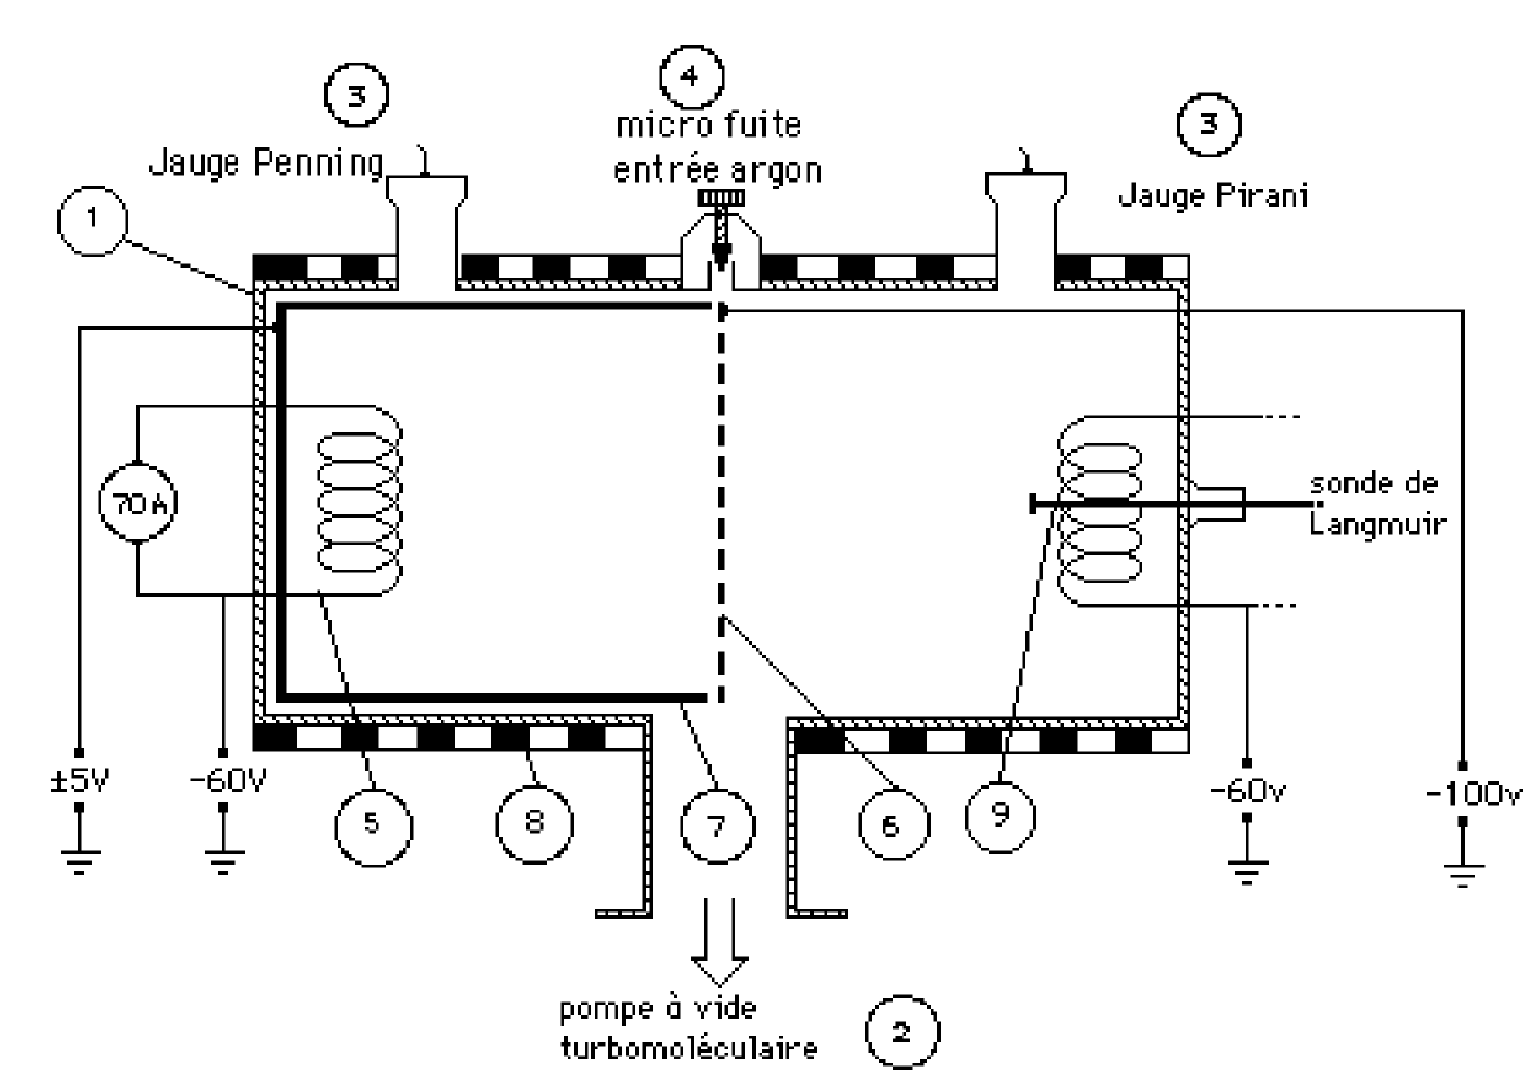
\includegraphics[width=12cm]{figures/experimental-setup.png}
    \caption{The experimental setup}
    \label{fig:experimental_setup}
\end{figure}